\chapter{LGT: Lattice without Fermions}\label{ch:preliminaries}

Physically, QFT is defined on a 4D Minkowskian space-time. In LGT 
the 4D space-time is instead equipped with a Euclidean metric, which is 
related to the original metric via a \index{rotation!Wick}{\it Wick rotation}
\begin{equation}
  t\to i\tau.
\end{equation} 
Therefore we will work with a Euclidean metric
and use downstairs summation indices. 
We will also use {\it natural units}\index{units!natural}
$\hbar=c=k_B=1$. In natural units, every physical
quantity has units of some power of length. For example
time has units of length, while energy, mass, and momentum
have units of inverse length. 
We first work in the continuum, then 
discretize the theory by defining the lattice.

\section{Local gauge symmetries}

Local gauge symmetries play a central role in the SM. 
Starting from a Lagrangian that depends on the derivatives of
some field, the requirement of local gauge invariance suggests that
we introduce a \index{gauge!field}{\it gauge field}. 
This gauge field allows one to define a {\it covariant derivative} 
\index{covariant derivative} whose transformation law will 
respect the local gauge symmetry.
Excitations of the gauge field are gauge bosons,
which are the force-carrying particles of the SM.

As an example consider $N_c$ complex scalar fields $\phi_{i}(x)$ equipped with 
a global $\SU(N_c)$ symmetry. The Lagrangian is
\begin{equation}\label{eq:LagrM}
  \Lagr_{M}=-\partial_{\mu}\phi^{\dagger}(x)\partial_{\mu}\phi(x)
                +m^{2}\phi^{\dagger}(x)\phi(x),
\end{equation}
where $\phi(x)$ is the $N_c$-dimensional vector formed by these fields.
$\Lagr_{M}$ becomes invariant under local $\SU(N_c)$ transformations, i.e. 
transformations of the form
\begin{equation}\label{eq:fxform}\index{gauge!transformation}
  \phi(x)\to U(x)\phi(x),
\end{equation}
where $U(x)\in \SU(N_c)$, when one replaces the partial derivative by the 
covariant derivative $D_\mu$, which transforms as
\begin{equation}\label{eq:dxform}
  D_\mu(x)\to U(x) D_{\mu}(x)U^{\dagger}(x).
\end{equation}
We define
\begin{equation}\label{eq:covariantderivative}
  D_{\mu}(x)\equiv\partial_{\mu}+A_{\mu}(x), \qquad 
       A_{\mu}(x)\equiv-igA^{a}_{\mu}(x)T^{a},
\end{equation}
where $g$ is the bare coupling constant, $A_{\mu}(x)$ is the gauge field, and 
$T^{a}$, $a=1,\dots,N^2-1$, are the generators of the $\SU(N_c)$ Lie algebra 
$\mathfrak{su}(N_c)$. For notational convenience we now suppress dependence
on $x$. 

\begin{proposition}{}{gaugecovar}
Using this definition of $D_\mu$, the gauge fields must change 
according to
$$A_{\mu}\to U A_{\mu}U^{\dagger}-(\partial_{\mu}U)U^{\dagger}.$$
%If the covariant derivative transforms as $D_\mu\to U D_\mu U^\dagger$
%under a gauge transformation, then the vector potential must
%transform as $A_\mu\to U A_\mu U^\dagger-(\partial_\mu U)U^\dagger.$
  \begin{proof} The transformed $D$ can be written
  $U D_\mu U^\dagger=\partial_\mu'+A_\mu'$. Solving for $A_\mu'$ gives
    \begin{equation*}
    \begin{aligned}
         A_\mu'
         &=U(\partial_\mu+A_\mu)U^\dagger-\partial_\mu\\
         &=U(\partial_\mu U^\dagger)
               +U A_\mu U^\dagger-\partial_\mu\\
         &=\partial_\mu-(\partial_\mu U)U^\dagger
               +U A_\mu U^\dagger-\partial_\mu\\
         &=U A_\mu U^\dagger
                -(\partial_\mu U)U^\dagger.      
    \end{aligned}
    \end{equation*}
  \end{proof}
\end{proposition}

The gauge field becomes dynamic by adding the kinetic part
\begin{equation}\label{eq:lagrkin}
  \Lagr_G=\frac{1}{4} F_{\mu\nu}^{a}F_{\mu\nu}^{a}
         =-\frac{1}{2g^2}\tr F_{\mu\nu}F_{\mu\nu},
\end{equation}
where 
\begin{equation}\label{eq:fieldstrength}
          F_{\mu\nu}^a\equiv \partial_\mu A_\nu^a-\partial_\nu A_\mu^a
                        +gf^{abc}A_\mu^b A_\nu^c,\qquad
  F_{\mu\nu}\equiv-igF_{\mu\nu}^aT^a,
\end{equation} 
and $f^{abc}$ are the structure constants of $\SU(N_c)$.
$\Lagr_{G}$ is also invariant 
under the transformation of \equatref{eq:dxform}. One way to see this
is to use the following fact.
\begin{proposition}{}{fieldtensor}
  $$F_{\mu\nu}=\left[D_\mu,D_\nu\right].$$
  \begin{proof}
    Use the definition of $D_\mu$ and apply the above commutator to some
    field $\psi$. We get
    \begin{equation*}
    \begin{aligned}
      \left[D_\mu,D_\nu\right]\psi
         &=(\partial_\mu+A_\mu)(\partial_\nu\psi+A_\nu\psi)
                     -(\mu\leftrightarrow\nu)\\
         &=\partial_{\mu\nu}\psi+\partial_\mu A_\nu\psi
           +A_\nu\partial_\mu\psi+A_\mu\partial_\nu\psi
           +A_\mu A_\nu\psi-(\mu\leftrightarrow\nu)\\
         &=\partial_\mu A_\nu\psi-\partial_\nu A_\mu\psi
           +\left[A_\mu,A_\nu\right]\psi\\
         &=-ig\left(\partial_\mu A_\mu^a-\partial_\nu A_\mu^a\right)T^a\psi
           -ig^2A_\mu^bA_\nu^cf^{bca}T^a\psi\\
         &=-ig\left(\partial_\mu A_\mu^a-\partial_\nu A_\mu^a
                    +gf^{abc}A_\mu^bA_\nu^c\right)T^a\psi\\
         &=F_{\mu\nu}\psi.
    \end{aligned}
    \end{equation*}
  \end{proof}
\end{proposition}

Taken altogether, the gauge-invariant, dynamical, 
scalar theory is described by the Lagrangian
\begin{equation}
  \Lagr=-(D_\mu\phi)^\dagger D_\mu\phi
                +m^2\phi^\dagger\phi
                -\frac{1}{2g^2}\tr F_{\mu\nu}F_{\mu\nu}.
\end{equation}
We would like
to point out that the definitions~\eqref{eq:covariantderivative} and
\eqref{eq:fieldstrength} are somewhat different than the convention
of many QFT books such as Srednicki~\cite{srednicki_quantum_2007}.
An advantage of the convention we have taken, which is also used in, 
for instance, Montvay and
M\"unster~\cite{montvay_quantum_1994}, is that one can explicitly see the
dependence of the Lagrangian~\eqref{eq:lagrkin} on the coupling. 

In this chapter we will be primarily interested in a theory with 
$\Lagr_G$ only and gauge group $\SU(N_c)$; such a theory is referred
to as {\it pure}\index{gauge!pure} $\SU(N_c)$.
Often the gauge particles of pure $\SU(N_c)$ theories are referred
to as ``gluons," even when $N_c\neq 3$. Because it
is non-Abelian, it has nonzero structure constants, which means it
contains self-interactions of the form $AAA$ and $AAAA$. 
These self-interactions are responsible for confinement, which we discuss
further in the next section. 
For the purpose of a lattice study,
it is helpful to look at a non-Abelian theory, which
has a well-defined continuum limit.

\section{Lattice regularization}\label{sec:latreg}
We now define QFT on a lattice. Let $N_{1},N_{2},N_{3},N_{4}
\in \N$. The {\it lattice} ${\LAT}$ is defined by
\begin{equation}
  {\LAT}\equiv\{x\,|\,x_\mu=a\,n_\mu,\,n_\mu\le N_\mu,\,
      \mu=1,2,3,4\}.
\end{equation}
Here $a$ is called the \index{lattice spacing}{\it lattice spacing}. 
After our Wick rotation, we identify $N_1$, $N_2$, and $N_3$
as the extensions of the lattice in the spatial directions,
and $N_4$ is taken to be the extension in the Euclidean time 
direction. Matter fields and gauge 
transformations are defined on the \index{site} {\it sites} $x\in\LAT$. We shall 
take the lattice to have periodic boundary conditions (BCs), i.e.
\begin{equation}\label{eq:PBC}
  x+aN_{\mu}\hat{\mu}=x,
\end{equation}
where $\hat{\mu}$ is the unit vector in the direction indicated by $\mu$. 
Since the lattice is discrete, one must replace partial derivatives 
by finite differences\footnote{The finite difference \equatref{eq:dertodiff},
known as the {\it central difference}\index{central difference},
exhibits errors in even powers of $a$, which you can show by Taylor
expanding $f(x+a\hat{\mu})$ and $f(x-a\hat{\mu})$ about $x$.}, 
\begin{equation}\label{eq:dertodiff}
  \partial_\mu f(x)\to\Delta_{\mu}f(x)\equiv\frac{f(x+a\hat{\mu})
                                                   -f(x-a\hat{\mu})}{2a},
\end{equation}
and similarly replace integrals with sums,
\begin{equation}\label{eq:inttosum}
  \int \dd[4]{x}\to a^4\sum_x.
\end{equation}
Moreover the BCs~\eqref{eq:PBC} imply for every direction
that the momentum is discretized as
\begin{equation}
  p_\mu=\frac{2\pi}{a}\frac{n_\mu}{N_\mu},
\end{equation}
which means that momentum space integrals must also be replaced by
sums
\begin{equation}
  \int\frac{\dd[4]{p}}{(2\pi)^4}\to
  \frac{1}{a^4N_1N_2N_3N_4}\sum_p. 
\end{equation}
Putting QFT on a lattice regularizes\footnote{Maybe it is worth
emphasizing here that this is a non-perturbative regularization. 
In particular, when one normally regularizes in QFT, it's because
one encounters some divergence when doing a perturbative
expansion. One then defines a regulator to parameterize this
divergence and tries to figure out which Feynman diagrams 
cancel it. In the case of LGT, the regulator is not tied to
any perturbative expansion.} the theory. 
To see this, consider a field $\phi$ defined on the lattice. 
Its Fourier transform
\begin{equation}
  \widetilde{\phi}(p)=a^4\sum_xe^{-ipx}\phi(x)
\end{equation}
is periodic in momentum space, which gives us the correspondence
$p_\mu\leftrightarrow p_\mu+2\pi/a$. Hence we can restrict
momenta to the \index{Brillouin zone}{\it first Brillouin zone},
\begin{equation}
 -\frac{\pi}{a}<p_\mu\le\frac{\pi}{a}
\end{equation}
and one obtains a UV cutoff $|p_\mu|\le\pi/a$.

Now we define the building blocks necessary to construct paths on the 
lattice. The directed {\it link}\index{link} connects $x$ with the 
neighboring point $x+a\hat{\mu}$, and its corresponding {\it link variable} 
$U_\mu(x)\in \SU(N_c)$ is defined by
\begin{equation}\label{eq:linkVariable}
  U_\mu(x)=e^{-aA_{\mu}(x)},
\end{equation}
where $A_{\mu}(x)\in\su(N_c)$. A link variable is
depicted in Fig.~\ref{fig:links} (left).
We associate to any path $\mathcal{C}$ 
the ordered product of its link variables $U(\mathcal{C})$. 
If we follow a path and then reverse our steps, we should end
up back where we started; hence
\begin{equation}
  U_{-\mu}(x+a\hat{\mu})U_\mu(x)=\id.
\end{equation}
Furthermore $U^\dagger(x)U(x)=\id$, so we can see the effect
of the dagger on link variables:
\begin{equation}
  U_\mu^\dagger(x)=U_{-\mu}(x+a\hat{\mu}).
\end{equation}
Let $\mathcal{C}_{x}$ be a path on the lattice that originates and 
terminates at the point $x$. The corresponding {\it Wilson loop} is 
defined by \index{Wilson!loop}$\tr U(\mathcal{C}_{x})$. 
Under local gauge transformations, link variables 
transform as
\begin{equation}
  U_\mu(x)\to U(x)U_\mu(x)U^{\dagger}(x+a\hat{\mu}),\qquad
  U(x)\in\SU(N_c),
\end{equation}
which ensures the gauge invariance of Wilson loops.
Maybe at this point it is worth pointing out that link variables will
have a Lorentz index attached to them (they live on the links) but
gauge transformations do not (they live on the sites). A \index{plaquette}
{\it plaquette}, shown in Figure~\ref{fig:links} (middle), is the 
smallest Wilson loop, an oriented square of side length $a$ with 
corresponding link variable 
\begin{equation}
  \plaq_{\mu\nu}(x)=U_\mu(x)U_\nu(x+a\hat{\mu})
                        U^\dagger_\mu(x+a\hat{\nu})U^\dagger_\nu(x).
\end{equation}
Every link variable in 4D LGT is part of six plaquettes\footnote{In $n$
dimensions, each site $x$ has $n!/2(n-2)!$ positively oriented plaquettes 
with a link starting at $x$ and pointing away from it. This is equal to the
number of unique combinations of directions. Each link has $2(n-1)$ staples
attached to it.}. The remaining
three edges of any particular plaquette are shaped like
a staple; therefore we call the combination
\begin{equation}\begin{aligned}\label{eq:staple}\index{staple}
  U^\sqcup_\mu(x)=
  \sum_{\nu\ne\mu}\Big[
   &U_\nu(x)U_\mu(x+a\hat{\nu})U^\dagger_\nu(x+a\hat{\mu})\\
   &+U^\dagger_\nu(x-a\hat{\nu})U_\mu(x-a\hat{\nu})
                   U_\nu(x-a\hat{\nu}+a\hat{\mu})\Big]
\end{aligned}\end{equation}
the {\it staple matrix}. A 2D staple matrix is shown in
Fig.~\ref{fig:links} (right); alternatively one can view it
as one of the three terms in the sum~\eqref{eq:staple}.

\begin{figure}[t]
  \centering
  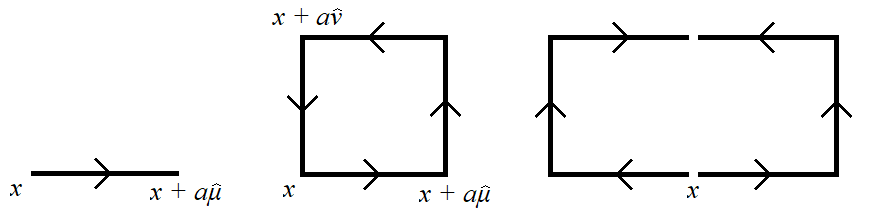
\includegraphics[width=0.9\linewidth]{figs/links.png}
  \caption{Left: A link variable. Middle: A plaquette. 
           Right: A staple matrix in 2D.}
  \label{fig:links}
\end{figure}

Plaquettes are used to construct the gauge-invariant $\SU(N_c)$ {\it Wilson
gauge action} \cite{wilson_confinement_1974}, given by
\begin{equation}\label{eq:wilsonaction}\index{Wilson!gauge action}\index{action!Wilson gauge}
    S_W\equiv\beta\sum\limits_{x;\,\mu<\nu}\left(1
         -\frac{1}{N_c}\Re\tr \plaq_{\mu\nu}(x)\right).
\end{equation}
The factor $\beta$ is given this name in analogy to the inverse temperature 
in statistical mechanics. Note that in this notation, the action has the
minimal value 0\footnote{This can be seen as follows: Go to a basis in which
$\plaq$ is diagonal. Since it is unitary, we see that its diagonal
entries must be pure phases. Hence $|\Re\tr\plaq|\leq N_c$.}. 
The Wilson action becomes identical with the
pure $\SU(N_c)$ action in the continuum limit because the plaquette is
directly related to the field tensor, which is proven in the following
proposition. 
\begin{proposition}{}{plaquette}
$$
U^\Box_{\mu\nu}(x)=\exp\left[-a^2F_{\mu\nu}(x)+\order{a^3}\right].
$$
  \begin{proof}
    Starting with the definition of the plaquette variable, we have
    \begin{equation*}\begin{aligned}
      U^\Box_{\mu\nu}(x)&=U(x,x+a\hat\nu)\,U(x+a\hat\nu,x+a\hat\nu+a\hat\mu)\\
               &~~~~\times U(x+a\hat\mu+a\hat\nu,x+a\hat\mu)\,U(x+a\hat\mu,x)\\
            &=\exp\left[aA_\nu(x)\right]\,
              \exp\left[aA_\mu(x+a\hat\nu)\right]\\
               &~~~~\times\exp\left[-aA_\nu(x+a\hat\mu)\right]\,
                \exp\left[-aA_\mu(x)\right]\\
            &=\exp\left[aA_\nu(x)\right]\,
               \exp\left[a\left( A_\mu(x)+a\partial_\nu A_\mu(x) \right)
                                 +\order{a^3}\right]\\
               &~~~~\times
               \exp\left[-a\left(A_\nu(x)+a\partial_\mu A_\nu(x) \right)
                                 +\order{a^3}\right]\,
               \exp\left[-aA_\mu(x)\right]\\
            &=\exp\left[aA_\nu+aA_\mu+a^2\partial_\nu A_\mu
                 +\frac{1}{2}\left[aA_\nu,aA_\mu\right]
                 +\order{a^3}\right]\\
            &~~~~\times\exp\left[-aA_\nu-a^2\partial_\mu A_\nu-aA_\mu
                 +\frac{1}{2}\left[-aA_\nu,-aA_\mu\right]
                 +\order{a^3}\right]\\
            &=\exp\left[a^2\partial_\nu A_\mu+a^2\left[A_\mu,A_\nu\right]
                 -a^2\partial_\mu A_\nu+\order{a^3}\right]\\
            &=\exp\left[-a^2F_{\mu\nu}+\order{a^3}\right].
    \end{aligned}\end{equation*}
    In the fourth step we applied the Campbell-Baker-Hausdorff formula and
    dropped the $x$ dependence for notational convenience, since at this
    step all the gauge fields depend on the same space-time point anyway.
    The fifth step uses another application of the Campbell-Baker-Hausdorff
    formula.
  \end{proof}
\end{proposition}
After some algebra, the connection between the Wilson action and the action
corresponding to \equatref{eq:lagrkin} becomes clear.
\begin{proposition}{}{wilsonCont} 
  $$S_W=-\frac{\beta}{4N_c}\sum_x a^4\tr F_{\mu\nu}(x)F_{\mu\nu}(x)
                  +\order{a^5}.$$
  \begin{proof} Using the definition~\eqref{eq:wilsonaction} and
    \propref{prp:plaquette} we have
    \begin{equation*}
    \begin{aligned}
      S_W&=\beta\sum_{x,\mu<\nu}\left(1-\frac{1}{N_c}\Re\tr 
            U_{\mu\nu}^\Box(x)\right)\\
         &=\beta\sum_{x,\mu<\nu}\left(1-\frac{1}{2N_c}\tr 
            \left[U_{\mu\nu}^\Box(x)+
            U_{\mu\nu}^\Box(x)^\dagger\right]\right)\\
         &=\beta\sum_{x,\mu<\nu}\left(1-\frac{1}{2N_c}\tr
            \left[2\id+\frac{a^4}{2}F_{\mu\nu}(x)^2
                  +\order{a^5}\right]\right)\\
         &=\beta\sum_{x,\mu<\nu}\left(-\frac{a^4}{2N_c}\tr F_{\mu\nu}(x)^2
                  +\order{a^5}\right)\\
         &=-\frac{\beta}{4N_c}\sum_x a^4\tr F_{\mu\nu}(x)F_{\mu\nu}(x)
                  +\order{a^5}.
    \end{aligned}
    \end{equation*}
    The cancellation of the $\order{a^2}$ term can be seen
    as follows: The role of the $\dagger$ in $\SU(N_c)$ is to take the inverse.
    For a path of link variables, this is the same as following the path
    in reverse.
    Following a plaquette in reverse just interchanges $\mu$ and $\nu$,
    which flips the sign of the leading term in the exponential
    of \propref{prp:plaquette} because $F_{\mu\nu}$
    is antisymmetric. Meanwhile the $\order{a^3}$ term must vanish
    since the exponent of $U_{\mu\nu}^\Box(x)$ is traceless. 
  \end{proof}
\end{proposition}

In the limit $a\to0$, the Wilson action coincides with the action
$S_G=\int \dd^4x\,\Lagr_G$ when one identifies 
\begin{equation}
  \beta=\frac{2N_c}{g^2}.
\end{equation}
Because of this identification, $\beta$ is also (besides $g$) sometimes 
referred to as the \index{coupling constant}{\it coupling constant}.

In \propref{prp:wilsonCont} we write the correction is $\order{a^5}$,
but actually only even powers of $a$ are permitted in the expansion.
This is not special to the Wilson action, but true of lattice actions
more generally. Indeed due to \equatref{eq:linkVariable}, you can
convince yourself that every $a$ comes attached to a Lorentz vector.
In most cases this is just $A_\mu$ in some direction, but in
\propref{prp:plaquette} we also see Lorentz indices emerge when
expanding, e.g., $A_\mu(x+a\hat{\nu})$. In such expansions, each
new Lorentz index also adds exactly one power of $a$. Hence there
is an exact correspondence between powers of $a$ and number of Lorentz 
indices. Therefore odd powers of $a$ are attached to odd numbers
of Lorentz indices. Such objects are parity-odd, and since the
action is parity-even, cannot appear in the expansion.

\section{The Haar measure}\label{sec:haar}\index{Haar measure}

We now restrict
our attention to lattices that have extension $N_1=N_2=N_3\equiv N_s$
and $N_4\equiv N_\tau$.
Expectation values of physical observables $X$ are given in 4D,
Euclidean, pure $\SU(N_c)$ LGT at zero temperature by
\begin{equation}\label{eq:0Tintegral}
  \ev{X}=\frac{1}{Z}\int\DD{U}e^{-S(U)}X(U),
\end{equation}
where the action is related to the Lagrangian by
\begin{equation}
  S=\int\dd[4]{x}\Lagr,
\end{equation}
$Z$ is the {\it partition function}
\begin{equation}
  Z\equiv\int\DD{U}e^{-S(U)},
\end{equation}
and the integration measure, the {\it Haar measure}, is
\begin{equation}
  \int\DD{U}\equiv\int\prod_{x,\mu}\dd{U_\mu(x)}.
\end{equation}
The quantities $X$ and $S$ appearing in the integral~\eqref{eq:0Tintegral}
are functionals of the configuration $U$, and this integral is
called a {\it functional integral}. The Haar measure is a product of
measures, one measure per link, each running over all possible values of
the link; in other words, the Haar measure runs over all possible
configurations\footnote{This is another advantage of the lattice formulation;
in the continuum, such integrals have an uncountably infinite dimension,
and it is hence not clear how to define them.}. The functional integral is therefore 
a weighted average of the observable $X$ over all possible configurations,
each configuration receiving a weighting factor $\int\DD{U}e^{-S}/Z$. 


We will now determine some properties of this measure. The gauge action is
invariant under gauge transformations, $U\to U'$. If we demand that the
functional integral is invariant under variable changes, we learn
\begin{equation}
  \int\DD U e^{-S(U)}
  =\int\DD U' e^{-S(U')}
  =\int\DD U' e^{-S(U)},
\end{equation}
which means
\begin{equation}
  \dd U_\mu(x)
   =\dd U_\mu(x)'=\dd\left(V(x)U_\mu(x)V(x+a\hat{\mu})^\dagger\right).
\end{equation}
Since $V(x)$ and $V(x+a\hat{\mu})$ can be chosen independently for an arbitrary
gauge transformation, it must be that
\begin{equation}\label{eq:haarcommute}
 \dd U=\dd(UV)=\dd(VU).
\end{equation}
This equation along with the normalization
\begin{equation}\label{eq:haarnorm}
  \int_{\SU(N_c)} \dd U=1
\end{equation}
are the defining properties of the Haar measure.

In what follows our integrals run over $\SU(N_c)$
and $V$ and $W$ are arbitrary $\SU(N_c)$ elements.
Using \equatref{eq:haarcommute} it follows for any 
integrable function $f$ on $\SU(N_c)$ that
\begin{equation}
  \int\dd Uf(U)=\int\dd Uf(VU)=\int\dd Uf(UV).
\end{equation}
Then using this equation, one can derive the following
useful integrals:
\begin{proposition}{}{}\label{prp:haar}
  Let $U\in\SU(N_c)$ in the fundamental representation. Then
  \begin{center}\begin{tabular}{lrcl}
  1. &$\int \dd U U_{ab}$ &=& 0;\\[1mm]
  2. &$\int \dd U U_{ab}U_{cd}$ &=& 0;\\[1mm]
  3. &$\int \dd U U_{ab}U^\dagger_{cd}$ 
       &=& $\frac{1}{N_c}\delta_{ad}\delta_{bc}$;\\[1mm]
  4. &$\int \dd U U_{ab}U_{cd}U_{ef}$ 
       &=& $\frac{1}{2 N_c}\epsilon_{ace}\epsilon_{bdf}$.
  \end{tabular}\end{center}
\end{proposition}
In \secref{sec:hqfe} we will encounter products of Wilson
loops that have one link in common. The third formula in
\propref{prp:haar} delivers the following equation, allowing
us to integrate out the common link in such situations:
\begin{equation}
  \int \dd U\tr VU\tr U^\dagger W=\frac{1}{3}\tr VW
\end{equation}

\section{Heavy quark free energy}\label{sec:hqfe}


When one thinks about the potential\footnote{At finite temperature
one distinguishes between potential energy and free energy since $F=U-TS$.}
energy between a static quark-antiquark pair, \index{static quark}
i.e. a pair of infinitely heavy quarks, one imagines
a Wilson loop $W(\mathcal{C}_{rt})$
where $\mathcal{C}_{rt}$ is a rectangular loop of side lengths 
$r$ and $t$ parallel
to the Euclidean time direction. When
viewing this Wilson loop in the temporal gauge, \index{gauge!temporal}
defined on the lattice by\footnote{In the Euclidean continuum theory,
the temporal gauge is defined by $A_4=0$.}
\begin{equation}
  U_4(x)=\id,
\end{equation}
one argues that
the edges parallel to the Euclidean time direction correspond to
a static quark-antiquark pair.
Then the {\it static quark potential}
\index{potential!static quark} $V(r)$ is defined by
\begin{equation}\label{eq:staticpotential}
  V(r)\equiv-\lim_{t\to\infty}\frac{1}{t}\log W(\mathcal{C}_{rt})  
\end{equation}
and gives the energy of the gauge field due to two color sources separated by
a distance $r$. 


We will argue the static quark potential has the form
\begin{equation}\label{eq:cornellpotential}
  V(r)=A+\frac{B}{r}+\sigma r,
\end{equation}
which is sometimes called the {\it Cornell potential}\index{potential!Cornell},
where $A$ and $B$ are constants and
$\sigma$ is the {\it string tension}\index{string!tension}. 
If the string tension is non-vanishing, then the potential scales linearly 
with $r$ in the large $r$ limit; 
this phenomenon has been observed in LGT 
simulations\footnote{Some studies are quoted in e.g.
Ref.~\cite{montvay_quantum_1994}.},
and we thus see LGT proffers an explanation of confinement.


The Coulomb-like term in \equatref{eq:cornellpotential} can be seen
mnemonically as follows. From \equatref{eq:fieldstrength}
one sees that the $\SU(N_c)$ field strength tensor has the same form
as the $\U(1)$ tensor, except for the last term, which is due to
$\SU(N_c)$ being non-abelian, and which comes with a factor $g$.
Hence in the small coupling limit, we recover the QED field
strength tensor. We know QED has a Coulomb term in its potential,
so we should a expect the $1/r$ term.


Conversely we argue for the linearly rising term in the strong
coupling limit. For arbitrary path $\mathcal{C}$ we expand the Wilson
loop expectation value as
\begin{equation}\label{eq:evWC}
  \ev{W_\mathcal{C}}=\frac{1}{Z}\int\DD U
    \exp\left(-\frac{\beta}{3}\sum_\square\Re\tr\left[\id-\plaq\right]\right)
    \tr\prod_{l\in\mathcal{C}}U_l,
\end{equation}
where the sum runs over plaquettes of some orientation and the product over
links in the Wilson loop. We factor out the sum over $\id$ appearing in the
both the numerator and the partition function to get
\begin{equation}\begin{aligned}
  \ev{W_\mathcal{C}}&=\frac{1}{Z'}\int\DD U
    \exp\left(\frac{\beta}{3}\sum_\square\Re\tr \plaq\right)
    \tr\prod_{l\in\mathcal{C}}U_l\\
                    &=\frac{1}{Z'}\int\DD U
    \exp\left(\frac{\beta}{6}\sum_\square\left(\tr \plaq+\tr
     U^{\square\,\dagger}\right)\right)
    \tr\prod_{l\in\mathcal{C}}U_l.
\end{aligned}\end{equation}
Now we expand the exponential:
\begin{equation}\begin{gathered}\label{eq:wilsonloopexpexpand}
    \exp\left(\frac{\beta}{6}\sum_\square\left(\tr \plaq+\tr
     U^{\square\,\dagger}\right)\right)~~~~~~~~~~~~~~~~~~~~
       ~~~~~~~~~~~~\\
    =\sum_{i,j=0}^{\infty}\frac{1}{i!j!}\left(\frac{\beta}{6}\right)^{i+j}
      \left(\sum_\square\tr\plaq\right)^i\left(\sum_{\square'}\tr
        U^{\square'\,\dagger}\right)^j.
\end{gathered}\end{equation}
Using this expansion, we can get the leading order contribution to the
denominator of \equatref{eq:evWC}. The zeroth order term is 1. The first
order term is zero due to the first statement of \propref{prp:haar}. Hence,
\begin{equation}
  Z'=1+\order{\beta^2}.
\end{equation}


To see where the linear behavior in \equatref{eq:cornellpotential} comes from,
we apparently need to apply this expansion to \equatref{eq:staticpotential}.
Hence we consider the rectangular contour $\mathcal{C}_{rt}$ with spatial
edge $r=an_r$ and $t=an_t$.
We will use the third statement in \propref{prp:haar} to calculate
the product of this exponential with the Wilson loop. 


The two plaquette sums
appearing in \equatref{eq:wilsonloopexpexpand} have opposite orientations, so
according to this Proposition, only one of those two sums can contribute when hitting
the Wilson loop.
\begin{figure}
  \centering
  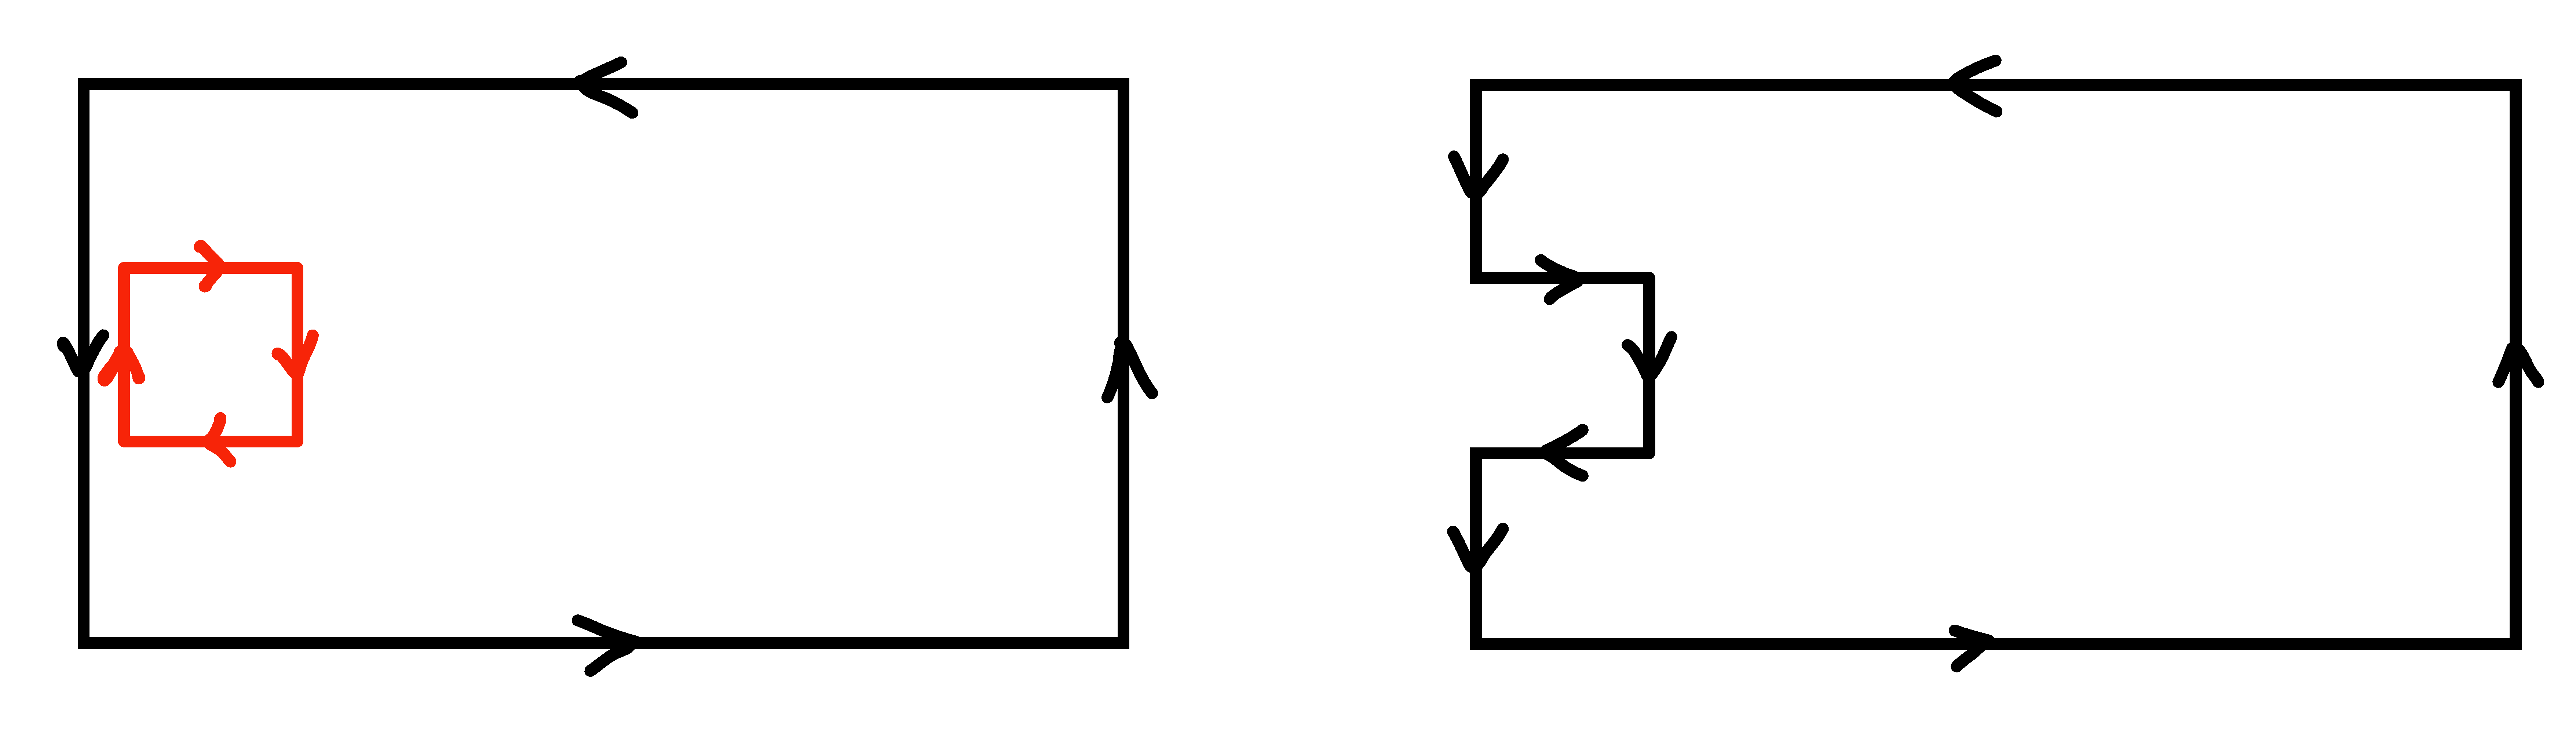
\includegraphics[width=0.9\linewidth]{figs/plaquetteTimesWilson.pdf}
  \caption{Integrating over the product of the Wilson loop $W(\mathcal{C}_{rt})$
           with an oppositely oriented plaquette. The resulting contour on the
           right comes with a factor 1/3 due to \propref{prp:haar}.}
  \label{fig:erasePlaquette}
\end{figure}
When a plaquette with non-vanishing contribution hits the loop,
the common link disappears, and the remainder of the plaquette is stitched to
the Wilson loop, as shown in \figref{fig:erasePlaquette}.
If in our sum there remains even one link that does integrate against a corresponding
plaquette, the integral will vanish according to statement 1 of
\propref{prp:haar}. Hence the only contributing terms are those terms in our
sum with a product of $n_A\equiv n_r n_r$ unique plaquettes that lie within
the boundary of the Wilson line. There are $n_A!$ such terms. Hence
\begin{equation}\begin{aligned}
  \ev{W(C_{rt})}
      &\approx\int\DD U\frac{1}{n_A!}\left(\frac{\beta}{6}\right)^{n_A}
            \left(\sum_\square\tr U^{\square\,\dagger}\right)^{n_A}
            \tr\prod_{l\in\mathcal{C}_{rt}}U_l\\
      &=\tr\id\left(\frac{\beta}{6}\right)^{n_A}\left(\frac{1}{3}\right)^{n_A}
\end{aligned}\end{equation}
If we look in the large $t$ limit and compare the above equation with 
\equatref{eq:staticpotential} we conclude at leading order in $\beta$
\begin{equation}
  V(r)\sim-\frac{r}{a^2}\log\left(\frac{\beta}{18}\right)\left(1+\order{\beta}\right)
          \equiv\sigma r,
\end{equation}
i.e. we identify this factor multiplying $r$ as the leading order expression
for the string tension. 


With static quarks, the consequence of this is that
the potential between a quark-antiquark pair diverges as you separate the pair.
With dynamical fermions, this potential energy eventually becomes larger than
the mass of a quark-antiquark pair, and it eventually becomes energetically
favorable to create such a pair out of the vacuum that binds to the two original
quarks forming two mesons. This phenomenon is known as 
{\it string breaking}\index{string!breaking}.


\section{Renormalization group and the continuum limit}
\index{renormalization!group}\index{limit!continuum}


In the limit $a\to0$, physical quantities $P$ should agree with experimental
results, which means they should become independent of $a$, ``forgetting"
about the lattice structure. Since $P$ depends in general also on $g$,
this means that changes in $a$ have to be compensated by changes in $g$
to keep the physics constant. More precisely, it must be that 
\begin{equation}
  \lim_{a\to0}P\Big(g(a),a\Big)=P_0
\end{equation}
where $P_0$ is the physical quantity's experimental value.
Both Callan~\cite{callan_broken_1970} and
Symanzik~\cite{symanzik_small_1970,symanzik_small-distance-behaviour_1971}
independently formulated the requirement of constant physics as
a differential equation
\begin{equation}\label{eq:RGflow}
  \left(\frac{\partial}{\partial\log a}
        +\frac{\partial g}{\partial\log a}
         \,\frac{\partial}{\partial g}\right)P=0. 
\end{equation}
(The RHS of this equation is more precisely
$\order{(a/\xi)^2\log(a/\xi)}$ for a lattice system
with correlation length $\xi$~\cite{montvay_quantum_1994}.)
Equation~\eqref{eq:RGflow} relates to a semi-group of scale 
changing transformations called the {\it renormalization group} (RG). 
The coefficient of the second term is called the {\it beta function},
\begin{equation}\label{eq:betafunction}\index{beta function}
  \beta\equiv-\frac{\partial g}{\partial\log a},
\end{equation}
and it measures how the bare\footnote{Usually in QFT one likes to label
a coupling that changes with some cutoff as a ``renormalized" coupling.
But in this case it really is the bare coupling that is changing with $a$.
One way to see this is that $a$ is not corresponding to any real-world
observable; the lattice spacing is just a calculational crutch. If changes
in a crutch need to be compensated by changes in another quantity,
the other quantity better also be a crutch, and indeed, bare quantities
are the ones that aren't measurable.}
coupling $g$ must change when $a$ changes.
The use of the symbol $\beta$ here is unfortunately a convention; it
is not to be confused with the coupling constant. It is usually clear
from context what is meant. 


In practice $\beta$ can be determined
from lattice perturbation theory. An explicit dependence of $g$ on $a$ is then
determined by solving the differential equation~\eqref{eq:betafunction}. 
For example the pure $\SU(N_c)$ lattice beta function\footnote{In a theory
with $N_f$ fermion flavors, the 1-loop contribution is
$$
  b_0=\left(\frac{11N_c}{3}-\frac{2N_f}{3}\right)\frac{1}{16\pi^2}.
$$
Hence when introducing fermions, at leading order, one loses asymptotic freedom
whenever $N_f\geq 11N_c/2$.} has been calculated 
up to 3-loop order in perturbation theory. It is given by
\begin{equation}\label{eq:blatgs}
  \beta_L(g)=-b_0g^3-b_1g^5-b_2^Lg^7+\order{g^{9}}
\end{equation}
where
\begin{equation}\label{eq:blat3loop}\begin{gathered}
  b_{0}= \frac{11}{3}\frac{N_c}{16\pi^2}, \qquad
  b_{1}= \frac{34}{3}\Bigg(\frac{N_c}{16\pi^2}\Bigg)^{2},\\
  b_{2}^{L}=\Bigg(-366.2+\frac{1433.8}{N_c^2}-\frac{2143.0}{N_c^4}\Bigg)
            \Bigg(\frac{N_c}{16\pi^2}\Bigg)^{3}
\end{gathered}\end{equation}
have been calculated at one-loop 
\cite{gross_d.j._ultraviolet_1973,politzer_reliable_1973}, two-loop 
\cite{belavin_calculation_1974,caswell_asymptotic_1974,jones_two-loop_1974},
and three-loop order~\cite{alle_three-loop_1997}, respectively.
The constants $b_0$ and $b_1$ are universal in the sense that they do not 
depend on the regularization scheme; however $b_2$ does depend on the
regularization scheme, with $b_2^L$ being the value using lattice
regularization. The RG equation on the lattice is
\begin{equation}
  \beta_{L}(g)=-a\dv{g}{a},
\end{equation}
and its solution is given by
\begin{equation}\label{eq:latRGEsoln}
  a\Lambda_{L}
   =\exp\Bigg(-\int^g\frac{\dd g'}{\beta_{L}(g')}\Bigg) \\
   =f_{as}\big(g^2\big)
   \equiv f_{as}^0\big(g^2\big)\sum\limits_{i=0}^{\infty}
     q_i\,g^{2i},
\end{equation}
where $q_0=1$, the other $q_i$ are coefficients that can be, in 
principle, calculated perturbatively, and
\begin{equation}\label{eq:f0}
   f_{as}^0\big(g^2\big)\equiv\exp\Bigg(-\frac{1}{2b_{0}g^2}\Bigg)
    (b_{0}g^{2})^{-b_{1}/2b_{0}^{2}}.
\end{equation}
In fact from \equatref{eq:blatgs} and \eqref{eq:blat3loop}, one obtains
\begin{equation}\label{eq:q1value}
  q_1=\frac{b_{1}^{2}-b_{2}^{L}b_{0}}{2b_{0}^{3}}=
  \begin{cases}
     0.08324 & \text{for}\ \SU(2) \\
     0.18960 & \text{for}\ \SU(3).
  \end{cases}
\end{equation}
The integration constant $\Lambda_{L}$ has units of mass and is called the
{\it lattice $\Lambda$-parameter}.
From \equatref{eq:latRGEsoln} one sees that
\begin{equation}\label{eq:llat}
  \Lambda_L=\lim_{g\to0}\frac{1}{a}f_{as}^0\big(g^2\big).
\end{equation}

\begin{figure}
  \centering
  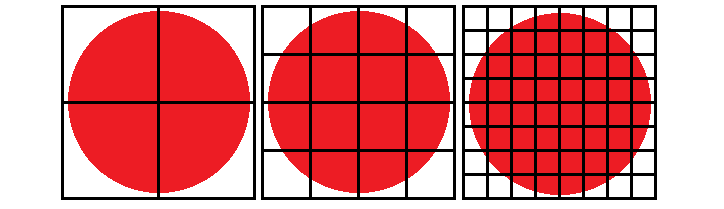
\includegraphics[width=0.9\linewidth]{figs/continuumlimit.png}
  \caption{A schematic representation of the continuum limit. The
           red object represents some physical quantity. As the
           images progress to the right, the lattice spacing decreases
           relative to the physical length, and the bare coupling
           becomes weaker.}
  \label{fig:climit}
\end{figure}

The fact that pure $\SU(N_c)$ theory has a negative beta function
\eqref{eq:blatgs} has a profound physical implication. In particular 
when we invert \equatref{eq:latRGEsoln} keeping only universal
terms, we find
\begin{equation}\label{eq:rgesoln}
  g(a)^{-2}=b_0\log\left(a^{-2}\Lambda_L^{-2}\right) 
            +\frac{b_1}{b_0}\log\log\left(a^{-2}\Lambda_L^{-2}\right)
            +\order{1/\log\left(a^2\Lambda_L^2\right)}.
\end{equation}
Two consequences are that the coupling\footnote{In the context of
QFT, we usually express a renormalized $g$ as a function of some
energy scale instead of $a$. This is called the 
{\it running coupling}\index{running coupling}. Sometimes also physicists
like to think of the interaction strength in terms of
$$
\alpha\equiv\frac{g^2}{4\pi}.
$$}
$g(a)$ is driven to zero
as $a$ approaches zero, which is known as 
\index{asymptotic freedom}{\it asymptotic freedom}, while at low energies,
$g(a)$ becomes too large for reliable perturbative analysis.

From \equatref{eq:latRGEsoln} we see that taking $g\to0$ drives $a\to0$.
However the limit $g\to0$ is not enough to ensure a well-defined continuum
limit. The physical size of the lattice is proportional to $a^4$, and hence
collapses to zero unless we also increase the number of sites. Therefore
we extrapolate to the continuum limit by calculating our observable
of interest at different values of the coupling constant, with the 
extensions $N_1$, $N_2$, $N_3$, and $N_4$ chosen so that the physical 
size of the lattice is large enough for a reliable calculation of 
the observable of interest. A schematic representation is shown in
Figure~\ref{fig:climit}. We note that two kinds of systematic uncertainty 
arise in this context. Namely, to what extent do finite lattice
spacing (which limits the smallest wavelength) and finite lattice
size (which limits the largest wavelength) affect our results?
These questions are discussed in detail in 
\secref{sec:refscales}.

\section{Finite temperature}\label{sec:finitetemp}

The functional integral for a 3D, 
pure $\SU(2)$ LGT system in contact with a thermal reservoir at 
temperature $T$ has the same structure, except that the corresponding 
action is
\begin{equation}\label{eq:Tintegral}
  S(T)=\int_0^{1/T}\dd{x_4}\int\dd[3]{x}\Lagr,
\end{equation}
and the Haar measure runs over fields that are periodic in the
$x_4$ direction. Because the functional integral for both systems is
formally the same, we interpret a 4D system with $N_s\gg N_\tau$ as
a 3D system at finite temperature, with $x_4$ running along a 
temperature direction rather than a time direction. 
The continuum limit of the finite temperature system corresponds
to $a\to0$ with $aN_s$ and $aN_\tau$ fixed. The {\it physical
temperature}\index{temperature} is seen to be
\begin{equation}\label{eq:latticeTemp}
  T=\frac{1}{aN_\tau}.
\end{equation}

From this equation, we see that at fixed lattice spacing, $T$ and $N_\tau$ are
inversely related. In particular, at fixed $a$, the limit $N_\tau=\infty$
delivers zero-temperature configurations. In practice, if we are interested in
zero-temperature physics, the best we can do is generate configurations with
negligibly small $T$. To judge whether $T$ is negligible, a good choice is
asking $T$ to be much smaller than the lightest bound state\footnote{You know
everything must be bound states because you're in the confined phase.}, 
which in $\SU(N_c)$ would be the lightest glueball. That $N_\tau$ needs to be
large enough to deliver a relatively small $T$ tends to make $T=0$ calculations
rather expensive, especially if you are additionally wanting to suppress size
effects, which requires also $N_s$ to be large.

\section{Scale setting I}\label{sec:refscales}\index{scale!setting}


Lattice computations deliver dimensionless quantities $L=\ell/a$, where 
$\ell$ is some physical length. $L$ is said to be expressed in {\it lattice
units}\index{units!lattice}, while $\ell$ is said to be in {\it physical
units}\index{units!physical}.\footnote{Another way to think about this
distinction is that $\ell$ is expressed in lattice units when $a=1$.}
The requirement that the theory has a 
well defined continuum limit means that for two length scales 
$\ell_i$ and $\ell_j$
\begin{equation}
  r_{ij}\equiv\frac{\ell_i}{\ell_j}=\lim_{a\to 0}\frac{L_i}{L_j}
        \equiv\lim_{a\to 0}R_{ij},
\end{equation}
i.e. in the continuum limit, length ratios attain their physical values.
Continuum limit extrapolations of a particular length $\ell_i$ therefore
depend on how one determines $R_{ij}$ and on the choice of the
{\it reference scale} or {\it reference length}\index{scale!reference} $\ell_j$. 
Choosing a reference scale to use for continuum limit extrapolation
is called {\it scale setting}, and commonly one says
``we set the scale with $\ell_j$." 


Calculation of the constants $R_{ij}$ is prone to nontrivial statistical and
systematic uncertainties. On the statistical side, observables, including
reference scales, come from randomly sampled field 
configurations\footnote{See \chref{ch:MCMC}.}, and increasing statistics
requires an increased computational effort. On the systematic side, there are
uncertainties coming from performing calculations at finite box size and how one
extrapolates to the continuum limit. Therefore it is desirable to set
the scale with a quantity that is computable with low numerical effort,
has small systematic uncertainties, and good statistical precision.


Eventually, it is important to tie whichever scale one picks to some
quantity that is experimentally accessible, for instance a particle
mass or a decay constant. A trick to successfully scale set in physical
units while keeping numerical effort low and precision high is to
compute a ratio like
\begin{equation}
\frac{\ell_{\rm nice}}{\ell_{\rm exp}}
\end{equation}
in the continuum once, where here $\ell_{\rm nice}$ is this nice scale with
high precision and low effort. Then for each ensemble, one can
easily compute $L_{\rm nice}$, giving you a good estimate for $a$ in physical units.


The choice of $\ell_{\rm exp}$ can also be a source of uncertainty. For example
experimental statistical and systematic uncertainties propagate into 
$\ell_{\rm exp}$. More subtly, there is a systematic uncertainty that arises
whenever there is a mismatch between the lattice Lagrangian and SM Lagrangian.
For example, we have been considering up to now pure $\SU(N_c)$ theories, which
are theories of $N_c$ colors of gluon only. Since we live in a world with all
kinds of other particles, there is no way to directly access pure $\SU(N_c)$ in
experiment. There are three approaches to somewhat circumvent this difficulty:
\begin{enumerate}
\item One can always report results as ratios of observables, never actually
connecting to some physical unit like MeV.
\item One can find indirect ways of relating quantities from physical and
unphysical theories. These are often model-dependent, and hence it is hard to
get a controlled, precise handle on the unphysical observable's value.
\item One can use scales that are less sensitive to the missing particles. For
example, most modern lattice calculations use at most the four lightest quarks,
arguing that the top and bottom quarks are too heavy to have a significant
effect, i.e. an effect detectable within the study's statistical precision.
\end{enumerate}
In the following subsections, we discuss some scales that have been used in pure
gauge simulations. We postpone the discussion of scales directly accessible in
experiment to \secref{sec:refscalesII}.


\subsection{String tension}\index{string!tension}


One of the first reference scales used in lattice calculations was the string
tension. The string tension is loosely related to physics experiment; it can be
extracted from Regge trajectories, but its value in MeV seems somewhat
model-dependent~\cite{smit_introduction_2002}, and hence it is difficult
to get a precise connection to physical units using this quantity.


\subsection{Deconfinement temperature}\index{temperature!deconfinement}
\index{phase transition!deconfining}


Another choice of scale for pure gauge systems is the 
{\it deconfining phase transition temperature}
\begin{equation}
  T_c=\frac{1}{a(\beta_c)\,N_\tau}.
\end{equation}
For $T<T_c$ gluons are bound into  glueballs, while 
at higher temperatures $T>T_c$ they exist in a gluon plasma. 
The deconfining phase transition is a second-order phase transition for 
$\SU(2)$~\cite{engels_critical_1996} and
and a first-order transition for $\SU(N_c)$ when $N_c>2$
~\cite{svetitsky_critical_1982}. 
The order parameter\footnote{We will argue this in \secref{sec:ploop}.} 
for this transition is the \index{Polyakov loop}
{\it Polyakov loop}\index{Polyakov loop},
\begin{equation}
  P(\vec{x})\sim\tr\prod_\tau U_4(\vec{x},\tau),
\end{equation}
which is a straight Wilson loop of length $N_\tau$ that is 
parallel to the Euclidean time 
axis and closes due to the periodic BCs. 
In practice, 
we determine $\beta_c$ by looking at plots of the Polyakov loop 
susceptibility,
\begin{equation}
  \chi=N_s^3\left(\ev{|P|^2}-\ev{|P|}^2\right), \qquad\qquad 
    P\equiv\sum\limits_{\vec{x}}P(\vec{x}),
\end{equation}
as a function of $\beta$ and estimating (in the infinite volume limit)
where it diverges. Numerical estimates
of $T_c$ are prone to systematic error because the simulations are
performed at finite lattice size while $T$ is only sharp in the infinite
volume limit. It is therefore necessary to extrapolate, for fixed $N_{\tau}$,
the dependence of $\beta_c(N_\tau)$ on the spatial size $N_s$ to the
infinite volume limit $N_s\to\infty$. Inverting $\beta_c(N_\tau)$ gives
$N_\tau(\beta)$, which is the 
\index{scale!deconfinement}{\it deconfinement scale}.


\subsection{Sommer scales}\index{scale!Sommer}

One of the difficulties of using $\sigma$ to set the scale is that it suffers
from relatively large systematic error, since it is defined in the limit that
the temporal edge of the Wilson loop goes to infinity.
In this section we will look at a scale that does not experience such a
systematic error.

We begin by computing the force\footnote{This differs from the usual
force definition by a minus sign.} corresponding to the Cornell
potential~\eqref{eq:cornellpotential},
\begin{equation}
  F(r)=\frac{\dd}{\dd r}V(r)
      =\frac{\dd}{\dd r}\left(A+\frac{B}{r}+\sigma r\right)
      =-\frac{B}{r^2}+\sigma,
\end{equation}
then multiply through by $r^2$ to make a dimensionless equation
\begin{equation}
  r^2F(r)=-B+\sigma r^2.
\end{equation}
The {\it Sommer scale} is the distance $r_c$ such that
\begin{equation}
  r_c^2F(r_c)=c
\end{equation}
with $r_{1.65}\equiv r_0$. This choice of RHS corresponds to
about $r_0\approx 0.5$ fm, which is roughly where the static potential in the
Cornell parameterization is zero.

In lattice units, the Sommer scale $r_c$ is given by
\begin{equation}
  \frac{r_c}{a}=\sqrt{\frac{c+B}{\sigma a^2}}.
\end{equation}
Hence one can extract $r_c/a$ once one knows $B$ and $\sigma a^2$. The most
straightforward way to extract these is
to simply carry out a fit to $aV(r)$.

\subsection{Gradient and cooling scales}\label{sec:gradcool}


A reference scale due to L\"uscher \index{gradient flow}
\cite{luscher_properties_2010}\index{scale!gradient} involves using 
the {\it gradient flow}. We begin by introducing a
fictitious {\it flow time} $t$ and evolve the system
according to the evolution equation
\begin{equation}\label{eq:Wflow}
  \dot{V}_\mu(x,t)=-g^2V_\mu(x,t)\,\partial_{x,\,\mu}S[V(t)]
\end{equation} 
with initial condition
\begin{equation}
  V_\mu(x,0)=U_\mu(x).
\end{equation}
In the above, the $\SU(N_c)$ link derivatives are defined by
\begin{equation}\begin{aligned}
  \partial_{x,\,\mu}f(V)&\equiv
     i\sum_aT^a\frac{\dd}{\dd s}f\left(e^{itX^a}V\right)\Big|_{t=0},\\
    X^a(x',\mu')&\equiv
    \begin{cases}
       T^a & \text{if} (x',\mu')=(x,\mu)\\
       0   & \text{otherwise.}
    \end{cases}
\end{aligned}\end{equation}
L\"uscher showed that the gradient flow averages the gauge field
$A_\mu$ over a sphere with mean-square radius $\sqrt{8t}$ in 4D. Hence
$t$ has dimension length squared, and $\sqrt{8t}$ is interpreted
as the {\it smoothing range} of the flow.
From \equatref{eq:Wflow} we see that the gradient flow lowers the action. 
For pure $\SU(2)$ the link derivative of the action takes the simple form
\begin{equation}\label{eq:SU2gflow}
  g^2\partial_{x,\mu}S(V)=\frac{1}{2}
          \left(V_\mu^\Box(x)-V_\mu^\Box(x)^\dagger\right).
\end{equation}

After choosing an energy density discretization $E$ (for example
one might use the Wilson action) a scale is defined by choosing an
appropriate, fixed, dimensionless {\it target value} $y$ and integrating
the gradient flow equation until 
\begin{equation}\label{eq:tardef}
  y=t^2 E(t).
\end{equation}
As a function of $\beta$, a {\it gradient scale}\index{gradient flow!scale}
\begin{equation}\label{eq:s}
  s(\beta)=\sqrt{t(\beta)}
\end{equation}
scales like a length, provided that
\begin{enumerate}
  \item lattice sizes are chosen so that $aN_{\min}\gg \sqrt{8t}$,
        where $N_{\min}=\min\,N_i$
        for simulations on an $N_1N_2N_3N_4$ lattice;
  \item the target values are large enough so that $\sqrt{8t}\gg a$ 
        for the smallest used flow time; and
  \item the values of $\beta$ are large enough to be in the
        $\SU(N_c)$ scaling region.
\end{enumerate}
In contrast to the deconfinement scale, the computation of 
a gradient scale does not require fits or extrapolations.
The only remaining ambiguity is how to choose a target value.

An alternative to the gradient flow that is similar and 
algorithmically simpler is known as {\it cooling}. 
Cooling was introduced as part of an investigation of
topological charge in the 2D O(3) sigma model \cite{berg_dislocations_1981}.
Bonati and D'Elia showed that using cooling as a smoothing technique produces
similar results for topological observables as the gradient flow
for pure $\SU(3)$ LGT \cite{bonati_comparison_2014}.
In pure SU(2) a standard cooling step is\index{cooling}
\begin{equation}\label{eq:cool}
  V_\mu(x,n_c)=\frac{V^\sqcup_\mu(x,n_c-1)}
                    {\sqrt{\det V_\mu^\sqcup(x,n_c-1)}},
\end{equation}
where $n_c$ is the number of cooling steps. 
The update \eqref{eq:cool} minimizes the local contribution to the
action, so that the ``cooling flow" decreases the action. Like with
the gradient flow, one picks a target value and iterates 
\equatref{eq:cool} until
\begin{equation}
  y=t_c^2 E(t_c),
\end{equation}
and a {\it cooling scale}\index{scale!cooling} is given by
\begin{equation}\label{eq:u}
  u(\beta)=\sqrt{t_c(\beta)}.
\end{equation}


\subsection{The scaling region and the continuum limit}
\label{sec:sysa}


One desires to know the ratio $r_{ij}$ of two scales in
the continuum limit. In principle this could be estimated by simulating
very near to the continuum limit. 
The continuum limit of LGT is defined in the vicinity of a second order
phase transition in the bare coupling. Because the correlation length
diverges near critical points, subsequent configurations become more
correlated, and it requires more configurations to obtain effectively
independent data. This is called {\it critical slowing down}. 
In practice, one therefore calculates
$R_{ij}$ at multiple $\beta$ (hence multiple $a$) and extrapolates
the continuum limit result based on these data. We now discuss
two possible fitting forms for continuum limit extrapolation. 

Using the Wilson action, ratios of observables that have
units of length are known to scale as 
\begin{equation}\label{eq:stdscaling}
  R_{ij}\equiv\frac{L_i}{L_j}=\frac{\ell_i}{\ell_j}\Big(1+
                     \order{a^2\Lambda_L^2}\Big).
\end{equation}
In the continuum limit, ratios
of lengths approach their continuum limit values.
Sometimes corrections depending on $a$, such as in the equation above, are
referred to as \index{lattice artifact}{\it lattice artifacts}. 
In general the approach to the
continuum limit is thought to have lattice artifacts of power $p$
(RG considerations show that these $a^p$ artifacts are modified by
powers of logarithms~\cite{montvay_quantum_1994}) where $p$ 
depends on the lattice discretization.
The Wilson action in particular has $p=2$.
Equation~\eqref{eq:stdscaling} suggests a two-parameter fit of the form
\begin{equation}\label{eq:stdscalingfit}
  R_{ij}=r_{ij}+c_{ij}\,\left(\frac{1}{L_j}\right)^2,
\end{equation}
where $r_{ij}$ and $c_{ij}$ are the 
fit parameters. We will refer to this behavior 
\index{scaling!standard}
as {\it standard scaling}. 


If we carry out a naive continuum limit without changing the
extension of the lattice, its physical volume collapses to zero.
Ideally, calculations would be performed 
in\index{thermodynamic!limit|see{\emph{limit, thermodynamic}}}\index{limit!thermodynamic} 
the thermodynamic limit,
where $N_s\to\infty$ and $N_\tau\to\infty$, and then take the limit
$a\to0$. In practice, the infinite volume observable is determined
by simulating at fixed $\beta$ on lattices of several sizes, then
extrapolating to the thermodynamic limit.
For some observables, the dependence on finite lattice size is known
from theory. For example the critical coupling constant $\beta_c(N_\tau)$
is known~\cite{engels_critical_1996} to depend on $N_s$ as
\begin{equation}
  \beta_c(N_\tau,N_s)=\beta_c(N_\tau)+a_1(N_\tau)N_s^{a_2(N_\tau)}.
\end{equation}
The $N_s=\infty$ result $\beta_c(N_\tau)$ can then
be extracted from a fit of the three parameters $\beta_c(N_\tau)$,
$a_1(N_\tau)$, and $a_2(N_\tau)$.


\section{Topological charge on the lattice}\label{sec:toplat}

It may seem counter-intuitive that a well-defined notion of topology
exists at all on the lattice. By taking an open cover of the
lattice as the manifold (e.g., one can associate a hypercube to
each site, keeping periodic BCs) one can define a topological charge on the 
lattice; the non-trivial topology is contained in transition functions
connecting cells of the open cover. For example 
L\"uscher~\cite{luscher_topology_1982} showed
the existence of a well-defined topological charge, which approaches 
$Q$ in the continuum limit, for configurations with a small action
density, i.e., with
\begin{equation}
  \max\,\tr\left(\id-U^\Box\right)<\epsilon
\end{equation}
for some small $\epsilon>0$. The maximum is taken over all plaquettes.
Configurations not satisfying this inequality are called 
\index{exceptional configuration}{\it exceptional}. 
Since
\begin{equation}
  \ev{\tr\left(\id-U^\Box\right)}=\frac{3}{8}g^2+\order{g^4},
\end{equation} 
one sees that exceptional configurations become suppressed 
as the lattice spacing
decreases. In order for a configuration of one topological charge to
tunnel to another, it must pass through such an exceptional configuration;
hence as $g$ decreases (as $\beta$ increases), it becomes increasingly 
more difficult for a configuration to tunnel out of its topological sector. 
This phenomenon is sometimes called {\it topological freezing}.

Further definitions of topological charge on the lattice can be found 
in reviews such as the review by Kronfeld~\cite{kronfeld_topological_1988}.
For our definition of topological charge, we follow the example of 
\equatref{eq:Q} using the rule~\eqref{eq:inttosum}. It is reasonable to 
measure a topological charge on the lattice by
\begin{equation}\label{eq:QL}
  Q_L=a^4\sum_x q_L(x),
\end{equation}
where the sum is over all lattice sites and
\begin{equation}\label{eq:QLdensity}
  q_L(x) = -\frac{1}{2^9\pi^2}\sum\limits_{\mu\nu\rho\sigma=\pm 1}^{\pm 4}
         \tilde{\epsilon}_{\mu\nu\rho\sigma}
         \tr U^\Box_{\mu\nu}(x)U^\Box_{\rho\sigma}(x).
\end{equation}
Here $\tilde{\epsilon}=\epsilon$ for positive indices while
$\tilde{\epsilon}_{\mu\nu\rho\sigma}=
  -\tilde{\epsilon}_{(-\mu)\nu\rho\sigma}$ for negative indices.
The summation over backwards indices along with the definition of
$\tilde{\epsilon}$ ensures $q_L$ has negative parity.
The restriction of generated configurations to a subset with some fixed
topological charge is what we mean by \index{topological!sector}
{\it topological sector}.
The lattice expression for the topological susceptibility is
\begin{equation}
  \chi_L=a^4\sum_x\ev{q_L(x)q_L(0)}=\frac{1}{N^4}\ev{Q_L^2},
\end{equation}
where we have assumed a geometry $N\equiv N_1=N_2=N_3=N_4$
and utilized the translational invariance due to periodic BCs.

Lattice gauge theories typically experience
local fluctuations of the gauge fields, which are produced stochastically. 
These fluctuations blur the topological structure of the lattice, and 
must therefore be stripped away from the configuration before measuring 
$Q_L$. The signal is considerably improved by \index{smoothing}
{\it smoothing}, where one replaces each link by a local average of links; 
$Q_L$ is then constructed on the smoothed field. 

Standard cooling minimizes the local contribution
to the action, which forces a gauge field to take a more typical
(smoother) value given its neighbors.
As mentioned earlier, the gradient flow averages the gauge field over 
a neighborhood, and therefore also has a smoothing effect. 
Ideally, these methods work because they make local modifications,
which therefore leave the global topological charge relatively intact.
A delicate issue with these smoothing algorithms is that they can destroy 
physical instantons; in fact after protracted cooling, a lattice will
eventually be brought to $Q_L=0$. This happens because
exceptional configurations or \index{topological!dislocation}
{\it dislocations} do not allow
for a well-defined topological charge. A lattice can then change
its topological charge by passing through these exceptional configurations.
In practice, one cools just enough
that topological observables become {\it quasi-stable}, i.e. just
enough that they do not change after many additional cooling sweeps.

\section{The Polyakov loop}\index{Polyakov loop}\label{sec:ploop}

This section is dedicated to the Polyakov loop, an object of crucial
historical and scientific significance in lattice calculations. The
Polyakov loop is an order parameter of the confinement-deconfinement
transition in pure $\SU(N_c)$ LGT. Since pure $\SU(N_c)$ physics is the 
same as physics with infinitely heavy quarks, this was historically used
as a means of getting some insight about the QCD transition. Nowadays
the Polyakov loop has fallen out of favor for this purpose at physical
quark masses and lower~\cite{clarke_polyakov_2020}.

\subsection{The Polyakov loop and deconfinement}\index{deconfinement}
\index{phase transition!deconfinement}
We begin with a brief review of some relevant properties of the
Polyakov loop. For a theory with underlying $\SU(N_c)$ gauge group, we define
the Polyakov loop by\index{Polyakov loop}
\begin{equation}\label{eq:ploop}
  P_{\vec{x}}\equiv\frac{1}{N_c}\tr\prod_\tau U_4(\vec{x},\tau).
\end{equation}
Because of the trace and periodic BCs, the Polyakov loop is invariant under
gauge transformations. For the purpose of, for instance, data analysis, it
is convenient to define the spatial average of the Polyakov loop,
\begin{equation}\label{eq:ploopav}
  P\equiv\frac{1}{N_\sigma^3}\sum_{\vec{x}}P_{\vec{x}}.
\end{equation}
Finally, some quantities of interest to us are defined more
naturally using the untraced Polyakov loop, or {\it thermal Wilson line}, 
\index{Wilson!line} which is just
\begin{equation}\label{eq:untracedPolyakov}
  L_{\vec{x}}\equiv\prod_\tau U_4(\vec{x},\tau).
\end{equation}
Each of the above is also sometimes referred to as a Polyakov
loop, which can be confusing because the untraced Polyakov loop is not
gauge invariant.

We now specialize to $\SU(3)$. The Polyakov loop relates to $F_{q\bar{q}}$,
\index{free energy!quark-antiquark}
the color-averaged free energy of a static quark-antiquark pair in
equilibrium at temperature $T$ by
\cite{mclerran_monte_1981,mclerran_quark_1981}
\begin{equation}\label{eq:Fav}
  \exp\left[-\frac{F_{q\bar{q}}(r,T)}{T}\right] 
    =\ev{P_{\vec{x}}P^\dagger_{\vec{y}}},
     \qquad rT=\left|\vec{x}-\vec{y}\tinysp\right|/N_\tau.
\end{equation}
At low temperatures with static quarks, the Polyakov loop expectation value
$\ev{|P|}$ is zero. This can be seen from at least two viewpoints. First
note that at large $r$, $P_{\vec{x}}$ and $P_{\vec{y}}$ become essentially
uncorrelated; therefore one finds
\begin{equation}\label{eq:ploop_decouple}
  \ev{P_{\vec{x}}P^\dagger_{\vec{y}}}
    \approx\ev{P_{\vec{x}}}\ev{P^\dagger_{\vec{y}}}
    =\ev{P}\ev{P^\dagger}
    =\ev{P}\ev{P}^\dagger
    =\left|\ev{P}\right|^2
    \approx\ev{|P|^2},
\end{equation}
and from \equatref{eq:Fav} we can (at least schematically) write
something like
\begin{equation}
  \ev{|P|^2}\sim\exp\left[-\frac{F_{q\bar{q}}(\infty,T)}{T}\right]. 
\end{equation}
Since $F_{q\bar{q}}$ is growing linearly with separation at low temperatures
due to confinement, the RHS of the above equation is zero.\footnote{You may
wonder how we jumped from $|\ev{P}|^2$ to $\ev{|P|}^2$, since it is generally
speaking not mathematically permissible to move the absolute value inside the
expectation value. It turns out that in the infinite volume limit this is
permissible. The reason is that $\ev{(\Im P)^2}$
will approach zero in the thermodynamic limit. We
will demonstrate this in \secref{sec:ploopfss}.}.
Another viewpoint is as follows: $\ev{|P|}$ is zero due to the global
$\Z_3$ symmetry of the gauge action. In particular one can show
that the plaquette is unchanged when multiplying all temporal links in a
given time slice $x_4=t_0$ with the same element $z\in\Z_3$, i.e.
the gauge action is unchanged under
\begin{equation}
  U_4(\vec{x},t_0)\to zU_4(\vec{x},t_0).
\end{equation}
The Polyakov loop is in general changed by this transformation
because it winds around the time direction. However since the action remains
unchanged, one can write
\begin{equation}\label{eq:centerzero}
  \ev{P}=\frac{1}{3}\ev{P+zP+z^2P}=\frac{1}{3}\left(1+z+z^2\right)\ev{P}=0
\end{equation}
since the sum over the center elements is zero.

At higher temperatures the first equality of \equatref{eq:centerzero}
no longer holds. At the deconfinement temperature $\Td$, this center symmetry
is spontaneously broken, and $\ev{|P|}$ acquires a nonzero value, signalling
a finite static quark-antiquark free energy and hence deconfinement.
At finite $N_\sigma$, $\ev{|P|}$ has an inflection point at $\Td$, and
the slope at this point diverges in the infinite volume limit. The Polyakov
loop susceptibility, defined as
\begin{equation}\index{Polyakov loop!susceptibility}
  \chi_{|P|}=N_\sigma^3\left(\ev{|P|^2}-\ev{|P|}^2\right).
\end{equation}
exhibits a pronounced peak in a finite volume $N_\sigma^3\times N_\tau$ at
$T_c$. The peak height diverges in the infinite volume limit as
$\chi^{\rm max}_{|P|}\sim N_\sigma^3$, reflecting the first order nature of
the deconfinement phase transition in pure $\SU(3)$ gauge theory.

One can argue that, as far as susceptibilities go, it is the 
susceptibility of $\Re P$ rather than $|P|$ that more directly contains the
relevant physics. This point can be seen as follows:
By doing a hopping parameter expansion of the fermion determinant,
which is valid in the limit of heavy quarks, and by doing a strong
coupling expansion in the kinetic part, one finds the leading order
contributions
\begin{equation}
  S=S_G+S_F\approx\sum_{\vec{x},\vec{y}}\tr L_{\vec{x}}\tr L_{\vec{y}}^\dagger
          +h\sum_{\vec{x}}\left(\tr L_{\vec{x}}+\tr L_{\vec{x}}^\dagger\right),
\end{equation}
where $h$ is an effective coupling that we will treat like an external
field strength. The first term in the fermionic part is coming from loops
winding around the lattice in the positive temporal direction, while the
second term comes from loops oriented in the negative temporal direction.
With the action in this form, one can more easily see the analogy with
an Ising model solid subject to an external magnetic field.
The susceptibility is then by definition
\begin{equation}
  \chi=\frac{\partial^2\log Z}{\partial h^2},
\end{equation}
where
\begin{equation}
  Z=\int\DD U\,e^{-S(h;U)}
\end{equation}
is the partition function. We compute
\begin{equation}
  \frac{\partial Z}{\partial h}
      =\int\DD U\sum_{\vec{x}}
          \left(\tr L_{\vec{x}}+\tr L_{\vec{x}}^\dagger\right)e^{-S(h;U)}
      =Z\ev{\sum_{\vec{x}}
          \left(\tr L_{\vec{x}}+\tr L_{\vec{x}}^\dagger\right)}
\end{equation}
and similarly
\begin{equation}
  \frac{\partial^2 Z}{\partial h^2}
      =Z\ev{\left\{\sum_{\vec{x}}
          \left(\tr L_{\vec{x}}+\tr L_{\vec{x}}^\dagger\right)\right\}^2\,}.
\end{equation}
Hence
\begin{equation}\begin{aligned}
  \chi&=\frac{\partial^2\log Z}{\partial h^2}\\
      &=\frac{1}{Z}\frac{\partial^2 Z}{\partial h^2}
       -\frac{1}{Z^2}\left(\frac{\partial Z}{\partial h}\right)^2\\
      &=\ev{\big\{\big\}^2}-\ev{\big\{\big\}}^2\\
      &=N_\sigma^3\left(\ev{(\Re P)^2}-\ev{\Re P}^2\right).
\end{aligned}\end{equation}
So from this point of view, the susceptibility of $\Re P$ is what
falls out the most naturally from the effective Polyakov loop action.
According to Frithjof, looking at $\chi_{\,|P|}$ became popular because
in quenched QCD in the confined phase, one finds two sectors with
nonzero $\Im P$, and it is easier to just measure $|P|$ than to rotate
measurements in these two sectors back to the real axis.


\subsection{Free energy and Polyakov loop renormalization}

The static quark-antiquark free energy $F_{q\bar{q}}$ gives the free
energy that comes from placing an infinitely heavy $q\bar{q}$ pair into the QCD
medium. Being static, the only contribution to the internal energy should be the
static potential $V$. On the other hand, one can thermodynamically relate
$F_{q\bar{q}}$ and $V$ by $F_{q\bar{q}}=V-TS$, from which one concludes
\begin{equation}
  F_{q\bar{q}}(r,T=0)=V(r).
\end{equation}

The gauge-invariant, color-averaged Polyakov loop correlator can be decomposed
into (in general gauge-dependent) color singlet $F_1$ and color octet $F_8$
contributions\index{free energy!color singlet}\index{free energy!color octet}
\cite{mclerran_monte_1981,mclerran_quark_1981,nadkarni_non-abelian_1986}.
In particular
\begin{equation}\label{eq:channels}
  \exp\left[-\frac{F_{q\bar{q}}(r,T)}{T}\right]
  =\frac{1}{9}\exp\left[-\frac{F_1(r,T)}{T}\right]
   +\frac{8}{9}\exp\left[-\frac{F_8(r,T)}{T}\right],
\end{equation}
where
\begin{equation}\begin{aligned}
 \exp\left[-F_1(r,T)/T\right]
   &=\frac{1}{3}\ev{\tr L_{\vec{x}}L^\dagger_{\vec{y}}}\\
  \exp\left[-F_8(r,T)/T\right]
    &=\frac{9}{8}\ev{P_{\vec{x}}P^\dagger_{\vec{y}}}
     -\frac{1}{24}\ev{\tr L_{\vec{x}}L^\dagger_{\vec{y}}},
\end{aligned}\end{equation}
which clearly depend on the gauge.
For small distances ($rT\ll1$ and $r\ll1/\Lambda_{\text{QCD}}$) it can
be shown within zero temperature perturbation theory
\cite{kaczmarek_heavy_2002} that
\begin{equation}\label{eq:Fperturb}
  F_1(r,T=0)
            =-8F_8(r,T=0)+\order{g^4}
            =-\frac{g^2}{3\pi r}\left(1+\order{g^2}\right).
\end{equation}
The exponent in \equatref{eq:channels} is positive for the singlet channel
but negative for the octet channel in this limit, which means $F_1$ dominates,
and we find
\begin{equation}
  F_{q\bar{q}}-F_1=T\log 9.
\end{equation}
Therefore,
\begin{equation}\label{eq:Tlog9}
  \lim_{r\to0}~F_{q\bar{q}}-F_1=T\log 9\qquad\Forall T.
\end{equation}

The Polyakov loop requires a multiplicative renormalization. Polyakov was the
first to notice that the Polyakov loop renormalizes as~\cite{polyakov_gauge_1980}
\begin{equation}\label{eq:renploop}
  P\ren=Z(\beta)^{N_\tau}P,
\end{equation}
where $Z(\beta)$ is the renormalization of the gauge field, i.e. of
each link. The same year, it was proven renormalizable to all orders in
perturbation theory~\cite{arefeva_quantum_1980,gervais_slope_1980}. 
From \equatref{eq:Fav} we see that $F_{q\bar{q}}$ requires an
additive renormalization. We can write
\begin{equation}\label{eq:renFav}
  a\,F_{q\bar{q}}\ren=a\,F_{q\bar{q}}+c(\beta),
\end{equation}
and then by \equatref{eq:Tlog9} we can similarly write
\begin{equation}
  a\,F_1\ren=a\,F_1+c(\beta)
\end{equation}
with the same $c(\beta)$ for both. From \equatref{eq:Fav},
\eqref{eq:renploop}, and \eqref{eq:renFav} we can write
\begin{equation}
  c(\beta)=-2\log Z(\beta).
\end{equation}

We note in passing that, in general, composite operators made of Polyakov loops
require a separate 
renormalization~\cite{polyakov_gauge_1980,arefeva_quantum_1980,gervais_slope_1980,korchemsky_renormalization_1987}.
This includes, for instance, the Polyakov loop susceptibility.

In practice, renormalized Polyakov loops can be calculated using
the $q\bar{q}$ {\it scheme}~\cite{kaczmarek_heavy_2002}.\index{renormalization
scheme!$q\bar{q}$} The additive
renormalization is determined by matching the singlet free energy
to the zero temperature potential at short distances, i.e.
\begin{equation}
  c(\beta)=a\,V_{T=0}(r_s)-a\,F_1(r_s,T),
\end{equation}
where $r_s$ is one of the shortest distances. (Often it is better to take
the third or fourth shortest available distance because the shortest
distance suffers the most from lattice artifacts.) The renormalized
Polyakov loop is determined as follows:
By \equatref{eq:Fav} and \eqref{eq:ploop_decouple}
\begin{equation}
  \lim_{r\to\infty}F_{q\bar{q}}\ren(r,T)
             =-T\log\left|\ev{P}\right|^2+c(\beta)T.
\end{equation}
Moreover as the distance between the pair increases, this free energy
should approach that of two quarks that do not interact with each other, i.e.
\begin{equation}
  \lim_{r\to\infty}F_{q\bar{q}}\ren(r,T)=2F_q\ren(T),
\end{equation}
where $F_q$ is the free energy of a heavy, static quark in the thermal
medium. The renormalized Polyakov loop is then recovered from its
relationship to this free energy, namely
\begin{equation}
  P\ren=\exp\left[-\frac{F_q\ren(T)}{T}\right],
\end{equation}
and from the above three equations we finally find
\begin{equation}
  P\ren=\exp\left[-\frac{1}{2}\left(\log\left|\ev{P}\right|^2
                                             -c(\beta)\right)\right].
\end{equation}

Historically, the $q\bar{q}$ scheme was the first lattice renormalization
strategy for the Polyakov loop. A major drawback of the $q\bar{q}$ scheme
is that it requires some $T=0$ calculations, which are generally speaking
extremely expensive, as was explained in \secref{sec:finitetemp}.
Several years later, a cheaper alternative was introduced, the so-called {\it
direct renormalization procedure}\index{direct renormalization}
\cite{gupta_renormalized_2008}.\footnote{ In this paper, they also 
point out a condition under which a Polyakov loop can be
renormalized in multiple representations.
Let $P_R$ indicate a Polyakov loop computed in some
representation $R$. If both the bare and renormalized Polyakov loops 
in two representations $R$ and $R'$ satisfy
$$
P_R^{1/C_2(R)}=P_{R'}^{1/C_2(R')},
$$
where $C_2(R)$ is the quadratic Casimir computed in representation $R$,
they are said to satisfy {\it Casimir scaling}\index{Casimir!scaling}.
If Casimir scaling holds, it follows that $Z_R(\beta)=Z_{R'}(\beta)$.
Hence under Casimir scaling, one can take over a result from the fundamental
representation to another one.}

The idea of the direct renormalization procedure is
to iteratively construct the renormalized Polyakov loop at all temperatures
starting from some known renormalized Polyakov loop at a reference temperature.
\begin{enumerate}
  \item As input, we need $P\ren(T_0)$ at some reference temperature
  $T_0$ along with the corresponding bare $P$ for at least two $N_\tau$, 
  say $N_{\tau,1}$ and $N_{\tau,2}$. $P\ren$ could be fixed by, for example, 
  the $q\bar{q}$ scheme. From \equatref{eq:renploop} it follows that
  \begin{equation*}\begin{aligned}
  P\ren(T_i)&=Z(\beta_{i,1})^{N_{\tau,1}}P(\beta_{i,1},N_{\tau,1})\\
            &=Z(\beta_{i,2})^{N_{\tau,2}}P(\beta_{i,2},N_{\tau,2}),
  \end{aligned}\end{equation*}
  for any $i$, where $i$ indicates the iteration step. Hence our first use
  of this equation will be for $i=0$.
  \item Next, we need a measurement of $P$ at $N_{\tau,1}$, this time using the
  coupling $\beta_{i,2}$. In other words,
  $$
  \beta_{i+1,1}=\beta_{i,2}.
  $$
  This delivers a new temperature
  $$
  T_{i+1}=\frac{1}{a(\beta_{i,2})N_{\tau,1}}=\frac{N_{\tau,2}}{N_{\tau,1}}T_i.
  $$
  Again from \equatref{eq:renploop} it follows that
  $$
  P\ren(T_{i+1})=Z(\beta_{i,2})^{N_{\tau,1}}P(\beta_{i,2},N_{\tau,1}).
  $$
  We already have $Z(\beta_{i+1,1})=Z(\beta_{i,2})$ from step 1, so combined with 
  our measurement of $P$, we can compute $P\ren(T_{i+1})$. Knowing $T_{i+1}$, we get
  $\beta_{i+1,2}$ using \equatref{eq:latticeTemp}. 
  \item Finally, we need a measurement of $P$ at $N_{\tau,2}$ and $\beta_{i+1,2}$.
  Another application of \equatref{eq:renploop} along with our already
  computed $P\ren(T_{i+1})$ enables us to deduce $Z(\beta_{i+1,2})$.
  \item We now have the same equations as step 1 for $i+1$, which defines
  the iterative process. 
\end{enumerate}

We note that while this procedure is cheap and straightforward, step 3 exposes
a drawback, namely that $\beta_{i+1,2}$ has to be obtained by inverting
the function $a(\beta)$, and hence this scheme is in principle sensitive to the
parameterization of $a(\beta)$. 

The final, standard approach to renormalizing the Polyakov loop is
the use of the gradient flow. L\"uscher and Weisz showed perturbatively 
that the gradient flow maps configurations to smooth, renormalized 
fields~\cite{luscher_perturbative_2011}. The flow time that you
choose defines a renormalization scheme. It was mentioned above that the
standard multiplicative renormalization does not automatically renormalize
composite operators. Interestingly, lattice calculations seem to suggest
that this approach takes care of the Polyakov loop susceptibility
as well~\cite{datta_using_2016,bazavov_polyakov_2016}. What is also nice
about this approach is that to leading order in pure SU(3) gauge theory, 
the dependence of $P\ren$ on the flow time $t$ is known~\cite{datta_using_2016}
\begin{equation}
\log P\ren(T,t)=\frac{g^2(T)C_Fm_E}{8\pi T}+\order{g^4,g^4\sqrt{t}T},
\end{equation}
where $m_E=gT$ and $C_F$ is the quadratic Casimir in the fundamental
representation, given by \equatref{eq:casfund}.


\subsection{Finite size scaling}\label{sec:ploopfss}
In this section we discuss some finite volume effects related to the
Polyakov loop.
In the confined phase in pure $\SU(3)$, there are three sectors that $P$
clusters around in the complex plane, corresponding to the three roots
of unity. At finite quark mass, the real sector is preferred, which
can be seen for example in Fig.~\ref{fig:ploopScatter}. I've been told
that one can show from strong coupling arguments that the real sector
is preferred at finite quark mass, but do not understand that yet.
Also we expect $\ev{\Im P}=0$ at $\mu=0$. To see this note that for any
action symmetric under $U\to U^\dagger$, we have
\begin{equation}\begin{aligned}
  \ev{\Im P}&=\int\DD U\,e^{-S(U)}\Im P(U)\\
            &=\int\DD U^\dagger\,e^{-S(U^\dagger)}\Im P(U^\dagger)\\
            &=-\int\DD U\,e^{-S(U)}\Im P(U)\\
            &=-\ev{\Im P},
\end{aligned}\end{equation}
where in the third step we used the invariance of the Haar measure and
the action. Finite chemical potential breaks the $U\to U^\dagger$ symmetry,
so we cannot anticipate that $\ev{\Im P}$ will vanish anymore.

\begin{figure}
  \centering
  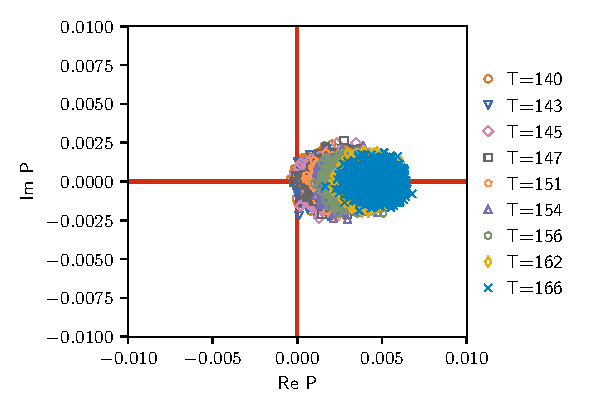
\includegraphics[width=0.7\textwidth]
          {figs/ploopScatter_betaDependl568ms80.pdf}
  \caption{Scatter plot of $P$ values for $56^3\times8$ HISQ configurations
           with $N_f=2+1$ at $m_s/m_l=80$. Temperatures are listed in MeV. 
           The real sector is preferred at finite quark mass.}
  \label{fig:ploopScatter}
\end{figure}

Let us discuss the large $N_\sigma$ behavior of some other quantities.
To simplify the notation a little, we introduce
\begin{equation}
x\equiv \Re P,~~~~y\equiv \Im P,~~~~\text{and}~~~~V\equiv N_\sigma^3.
\end{equation}
From the above discussion we have in this notation $\ev{y}=0$.
Note that $\ev{y^2}$ is generally not zero,
although it vanishes as $1/V$ with increasing V.
One can see $\ev{y^2}\neq0$ in Fig.~\ref{fig:ploopScatter}.

In particular one expects that $\ev{y^2}$ scales as
$1/V$. This is because in general $\log Z$ is proportional
to the free energy, so it is extensive and therefore scales as $V$;
therefore cumulants of extensive observables, which are coefficients in
the cumulant expansion, scale as $V$. It follows that the
susceptibility of an {\it intensive} observable scales as $1/V$,
and hence
\begin{equation}\label{eq:fssim}
  \ev{y^2}-\ev{y}^2 =\ev{y^2}=\frac{A}{V}
\end{equation}
for some volume-independent constant $A$. Indeed Fig.~\ref{fig:ImPvol} shows 
$\ev{y^2}$ scales linearly with $1/V$.

\begin{figure}
  \centering
  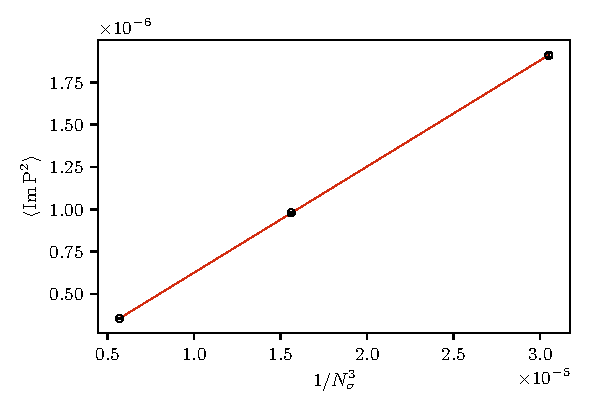
\includegraphics[width=0.7\textwidth]{figs/ImP2_voldepend.pdf}
  \caption{Volume dependence of the bare $\ev{(\Im P)^2}$ on $N_\tau=8$
           lattices with $\beta=6.445$, $m_s/m_l=80$, and $N_\sigma=32$, 40,
           and 56. The linear fit has
           $\chi^2/\text{d.o.f.}=0.11$.}
  \label{fig:ImPvol}
\end{figure}

It also follows from the scaling of terms in the cumulant expansion that
\begin{equation}\label{eq:fssre}
  \ev{x^2}-\ev{x}^2=\frac{B}{V}~~~~\text{and}~~~~\ev{x}=C
\end{equation}
for some volume-independent constants $B$ and $C$. By combining the two
equations in~\equatref{eq:fssre} one sees
\begin{equation}
  \ev{x^2}=C^2+\frac{B}{V}.
\end{equation}
In Figure~\ref{fig:FSSScalingOfSuscs} some of these relations are seen
to hold on $N_f=2+1$ HISQ lattices both above and below the chiral crossover.
We also see in this figure that $\ev{|P|}$ does not scale with volume 
in the same way as $\ev{\Re P}$ or $\ev{\Im P}$. This makes sense because
extensive quantities should scale linearly with the system size, but
absolute values are not linear. 

\begin{figure}
  \centering
  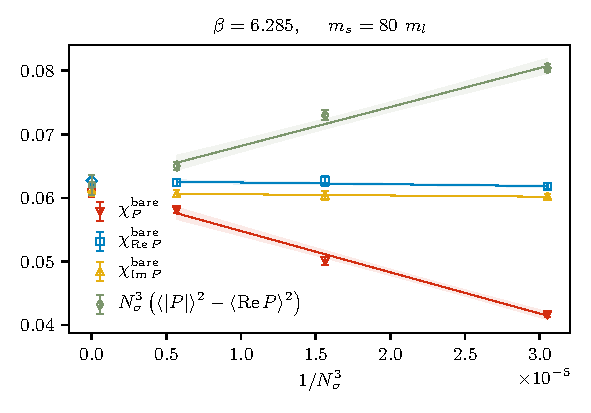
\includegraphics[width=0.45\textwidth]{figs/allSuscs_b6285.pdf}
  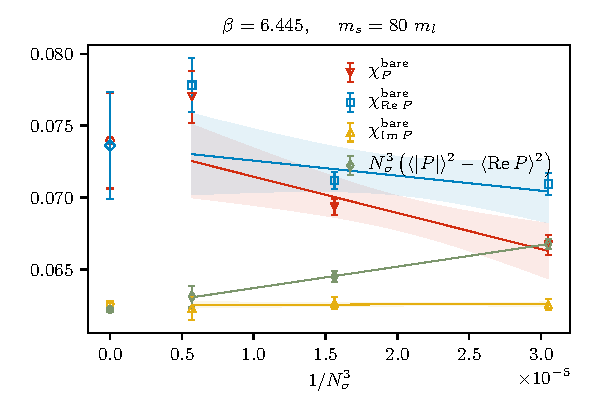
\includegraphics[width=0.45\textwidth]{figs/allSuscs_b6445.pdf}
  \caption{Finite size scaling of various susceptibilities
           for $N_\tau=8$, $m_s/m_l=80$ lattices for
           $\beta=6.285$ (left) and $\beta=6.445$ (right). Also shown are
           linear fits in $1/N_\sigma^3$ along with the
           infinite volume extrapolations.}
  \label{fig:FSSScalingOfSuscs}
\end{figure}


\begin{figure}
  \centering
  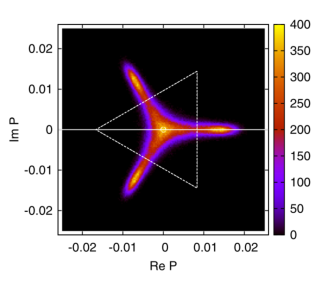
\includegraphics[width=0.45\textwidth]{figs/mercedesStar.pdf}
  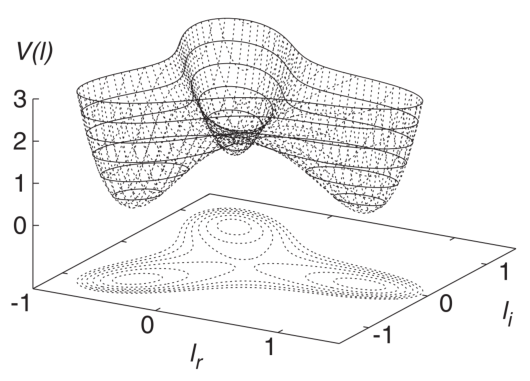
\includegraphics[width=0.45\textwidth]{figs/ploopPotential.pdf}
  \caption{{\it Left}: Heat map of Polyakov loop in complex plane, forming the
  Mercedes star pattern. The triangle indicates the phase boundaries.
  {\it Right}: Visualization of effective potential.}
  \label{fig:mercedesStar}
\end{figure}


\subsection{Effective potential}

In \figref{fig:ploopScatter} we see where the Polyakov loop likes to settle for
various temperatures. Both above and below the QCD crossover temperature, which
is about 155 MeV, it is found to cluster on the real axis.
This is a property of doing the simulation at finite quark mass. In pure SU(3),
the Polyakov loop settles differently in the complex plane; in particular it
clusters in three locations in the confined phase, forming a pattern sometimes
referred to as the {\it Mercedes star}\index{Mercedes star}.
An example of this behavior is shown in \figref{fig:mercedesStar} (left).



\bibliographystyle{unsrtnat}
\bibliography{bibliography}
